% !TeX root = ../tfg.tex
% !TeX encoding = utf8
%
%*******************************************************
% Capítulo 9. Clasificación ID
%*******************************************************

\chapter{Clasificación ID}\label{cap:clasificacion-id}

%\pendiente{introducción del capítulo: cinco arquitecturas preentrenadas con ajuste fino (ViT-B/16, ResNet-50, ConvNeXt-S, EfficientNetV2-S y Swin-S) y evaluación en el test ID}
En este capítulo se presentan los resultados y elección del mejor modelo para el resto de la experimentación. Se mostrarán las métricas obtenidas por los distintos modelos, y la matriz de confusión y las gráficas de pérdida, precisión y F1. Finalmente se presentará una conclusión general de esta parte de la experimentación.
\section{Comparación de los cinco modelos}\label{sec:comparacion-modelos}

\subsection{Resultados globales}\label{sec:modelos-global}

%\revisar{la tabla de exactitudes de las notas (salida de \texttt{resultados.txt}) se sustituye por la \cref{tab:modelos}, generada a partir de results\_fase1, con IC; las exactitudes coinciden salvo Swin-S (0,96870 $\to$ 0,9688) y ResNet-50 (0,89634 $\to$ 0,8964), por una imagen de diferencia; según results\_fase1/resumen.md, probablemente por la inferencia con precisión mixta (no comprobado)}

% Cifras clave (results_fase1): exactitud Swin-S 0,9688 [0,9658; 0,9717], ConvNeXt-S 0,9668
% [0,9635; 0,9700], EfficientNetV2-S 0,9538, ViT-B/16 0,9525, ResNet-50 0,8964. F1 macro: ConvNeXt-S
% 0,9086 y Swin-S 0,9082. IC por lámina 2-3 veces más anchos que por imagen.
% Swin-S − ConvNeXt-S: +0,0020, no significativa (McNemar p = 0,19, \cref{tab:mcnemar}).
En la \cref{tab:modelos} se aprecia cómo los dos mejores resultados han sido ofrecidos por las arquitecturas modernas, donde Swin-S presenta una exactitud de 0,9688, resultado muy similar al de ConvNeXt-S, que presenta 0,9668. Esta similitud puede deberse a que, a pesar de que ambos provienen de naturalezas distintas, redes convolucionales frente a Transformer, ConvNeXt emplea adaptaciones y elementos que eran originales de los Transformer (\cref{sec:convnext}). Por otro lado, Swin supera a ViT como era de esperar, pues el primero es una mejora del otro, en donde se diseñó para resolver la falta de jerarquía multiescala (\cref{sec:swin}). Por otro lado, EfficientNetV2-S, con una exactitud de 0,9538, muestra un resultado realmente competitivo, mostrando el potencial de combinar la búsqueda de arquitectura con el escalado~\cite{tan2021}, pero siendo ligeramente superado por ConvNeXt. Finalmente, de ResNet-50, arquitectura que supuso una revolución y el estado del arte en su momento, se aprecia que actualmente no puede competir con los modelos actuales, presentando la exactitud más baja, de 0,8964.
% Protocolos (tfg/executions/def1): clasificador.py (param0-3) frente a clasificador_svim.py (param4).
% Épocas descongeladas hasta la parada temprana (training_history.csv): ViT 28, ResNet 22, ConvNeXt 40,
% EfficientNetV2 51 (más 10 congeladas). Swin-S: 25/25 (slurm-123915.out), sin parada temprana.
La comparación entre Swin-S y los otros cuatro modelos no es homogénea, ya que no se entrenaron con el mismo protocolo (\cref{sec:learner}). El \texttt{vision\_learner} de fastai no admitía correctamente el Swin-S de timm, por lo que este se entrenó con un \texttt{Learner} genérico. Esto cambia varios elementos a la vez: la cabeza de clasificación (la de timm, sin el \emph{dropout} con $p = 0{,}5$ que añade fastai),
 la ausencia de una fase previa con el cuerpo de la red congelado, la tasa de aprendizaje (fija en $10^{-4}$, en lugar de la sugerida por \texttt{lr\_find}) y el número de épocas: 25 con \texttt{fit\_one\_cycle}, que se completaron sin que llegara a actuar la parada temprana, frente a 10 épocas congeladas y entre 22 y 51 descongeladas en los otros cuatro modelos, en los que el entrenamiento sí se detuvo por parada temprana. 
 Por tanto, las diferencias entre Swin-S y el resto no pueden atribuirse solo a la arquitectura. Aun así, Swin-S obtiene la mayor exactitud con un protocolo en apariencia menos favorable, sin búsqueda de la tasa de aprendizaje y con menos épocas, aunque no puede saberse si con el mismo protocolo que los demás mejoraría o empeoraría. Además, su diferencia con ConvNeXt-S (+0,0020) no es estadísticamente significativa (McNemar, $p = 0{,}19$; \cref{tab:mcnemar}),
  por lo que ambos modelos deben considerarse empatados y la elección de Swin-S no se apoya en una superioridad demostrada, si no en la mera casualidad de que ha ofrecido un resultado ligeramente mayor. 

% Generado por scripts/generar_tablas.py a partir de results_fase1/metricas_modelos.csv. No editar a mano.
\begin{table}
\centering
\scriptsize
\setlength{\tabcolsep}{3pt}
\caption{Clasificación de las 14 clases en el test ID (12.618 imágenes) con los cinco modelos: exactitud, F1 macro y \emph{balanced accuracy} (más alto es mejor).}
\label{tab:modelos}
\begin{tabular*}{\linewidth}{@{\extracolsep{\fill}}lccccccc}
\toprule
Modelo & Exactitud & IC 95\,\% (imagen) & IC 95\,\% (lámina) & F1 macro & IC 95\,\% (imagen) & IC 95\,\% (lámina) & \emph{Balanced acc.} \\
\midrule
Swin-S & 0{,}9688 & [0{,}9658; 0{,}9717] & [0{,}9589; 0{,}9768] & 0{,}9082 & [0{,}8919; 0{,}9224] & [0{,}8491; 0{,}9314] & 0{,}8907 \\
ConvNeXt-S & 0{,}9668 & [0{,}9635; 0{,}9700] & [0{,}9571; 0{,}9748] & 0{,}9086 & [0{,}8922; 0{,}9222] & [0{,}8583; 0{,}9322] & 0{,}8990 \\
EfficientNetV2-S & 0{,}9538 & [0{,}9500; 0{,}9575] & [0{,}9412; 0{,}9645] & 0{,}8719 & [0{,}8522; 0{,}8878] & [0{,}7906; 0{,}8963] & 0{,}8583 \\
ViT-B/16 & 0{,}9525 & [0{,}9487; 0{,}9559] & [0{,}9391; 0{,}9631] & 0{,}8740 & [0{,}8565; 0{,}8883] & [0{,}8007; 0{,}8966] & 0{,}8674 \\
ResNet-50 & 0{,}8964 & [0{,}8913; 0{,}9020] & [0{,}8687; 0{,}9166] & 0{,}7620 & [0{,}7434; 0{,}7796] & [0{,}6678; 0{,}7904] & 0{,}7375 \\
\bottomrule
\end{tabular*}

\smallskip
\parbox{\linewidth}{\scriptsize IC del 95\,\% por \emph{bootstrap} (1.000 remuestreos, semilla 0) sobre imágenes y sobre láminas (remuestreo de las 95 láminas). ConvNeXt-S se evalúa a 256\,px y el resto a 224\,px, cada uno con el preprocesado de su entrenamiento.}
\end{table}



\subsection{Curvas de entrenamiento y matrices de confusión}\label{sec:modelos-curvas}

% Para cada modelo: curvas de pérdida y métricas por época (Train_Validation_Results.jpg) y matriz
% de confusión en el test (Confusion_Matrix_TEST_*.jpg), de tfg/executions/def1/param0..4.

Las curvas de entrenamiento siguen un claro patrón en los modelos Swin-S, ConvNeXt-S, EfficientNetV2-S y ViT-B/16. En estos modelos, las curvas de pérdida en entrenamiento y validación decrecen de forma similar conforme aumentan las épocas, hasta llegar a un punto en el que la curva de validación deja de decrecer, lo que da lugar a dos situaciones: si crece, salta la parada temprana, y si se estanca, tardará más en saltar. Con los resultados en test y viendo la gráfica de error, los modelos carecen de sobreajuste.

Sin embargo, ResNet-50 presenta gráficas diferentes: en validación, la pérdida presenta un decrecimiento muy irregular, con muchos picos, y la exactitud y la F1 macro, en vez de tener un comportamiento asintótico, tienen un crecimiento casi lineal.

Una posible explicación, que planteamos como hipótesis, está en la interacción entre la política \textit{1cycle} y la parada temprana. En la fase descongelada, \texttt{fine\_tune} aplica \texttt{fit\_one\_cycle} sobre las 90 épocas previstas, con una fase de calentamiento en la que la tasa de aprendizaje crece durante aproximadamente el primer 30\,\% de las épocas (unas 27) y una fase posterior en la que decrece hasta casi cero. ResNet-50 se detuvo por parada temprana tras 22 épocas descongeladas, por lo que todo su entrenamiento se desarrolló en la fase de calentamiento, con una tasa de aprendizaje cada vez mayor. Con pasos tan grandes, los pesos cambian mucho de una época a otra y la pérdida de validación, muy sensible a los errores cometidos con alta confianza, oscila entre 0,864 y 1,086, mientras que la exactitud de validación crece de forma mucho más suave (de 0,869 a 0,906). A esto puede contribuir que ResNet-50 es la única de las cinco arquitecturas que emplea \emph{batch normalization}, cuyas estadísticas son sensibles a estos cambios bruscos. Además, la parada temprana salta precisamente por estas oscilaciones: la última mejora de la pérdida de validación superior a \texttt{min\_delta} se produjo en la época 11 (0,8685), ya que la de la época 14 (0,8644) no alcanza el umbral de 0,005, y diez épocas después se detuvo el entrenamiento.

Esto también explicaría el crecimiento casi lineal de la exactitud y de la F1 macro. La forma asintótica que muestran el resto de modelos se debe en gran parte a la fase final de la política \textit{1cycle}, en la que la tasa de aprendizaje baja y el modelo se estabiliza. ConvNeXt-S (40 épocas descongeladas) y EfficientNetV2-S (51) llegaron a esa fase, ViT-B/16 (28) apenas la alcanzó y Swin-S completó su ciclo de 25 épocas, mientras que ResNet-50 nunca llegó a ella. Por tanto, es probable que ResNet-50 estuviera lejos de converger y que su exactitud en test (0,8964) no refleje todo el potencial de la arquitectura, sino un entrenamiento interrumpido durante el calentamiento.
% Cifras: tfg/executions/def1/param1_*/training_history.csv (fase descongelada, épocas 0-21): valid_loss
% 0,8685 (época 11), 0,8644 (14), máx. 1,0864 (10); accuracy 0,8694 -> 0,9056 (máx.); F1 macro 0,696 -> 0,778.
% Calentamiento: fastai fine_tune -> fit_one_cycle(epochs, slice(base_lr/100, base_lr/2), pct_start=0.3);
% 0,3 x 90 = 27 épocas (implementación de fastai 2.7.19; no se ha registrado la tasa de aprendizaje por época).

Pérdida en test: 0,6788; exactitud en test: 0,9525.
\pendiente{análisis}

%\begin{figure}[tbp]
%  \centering
%  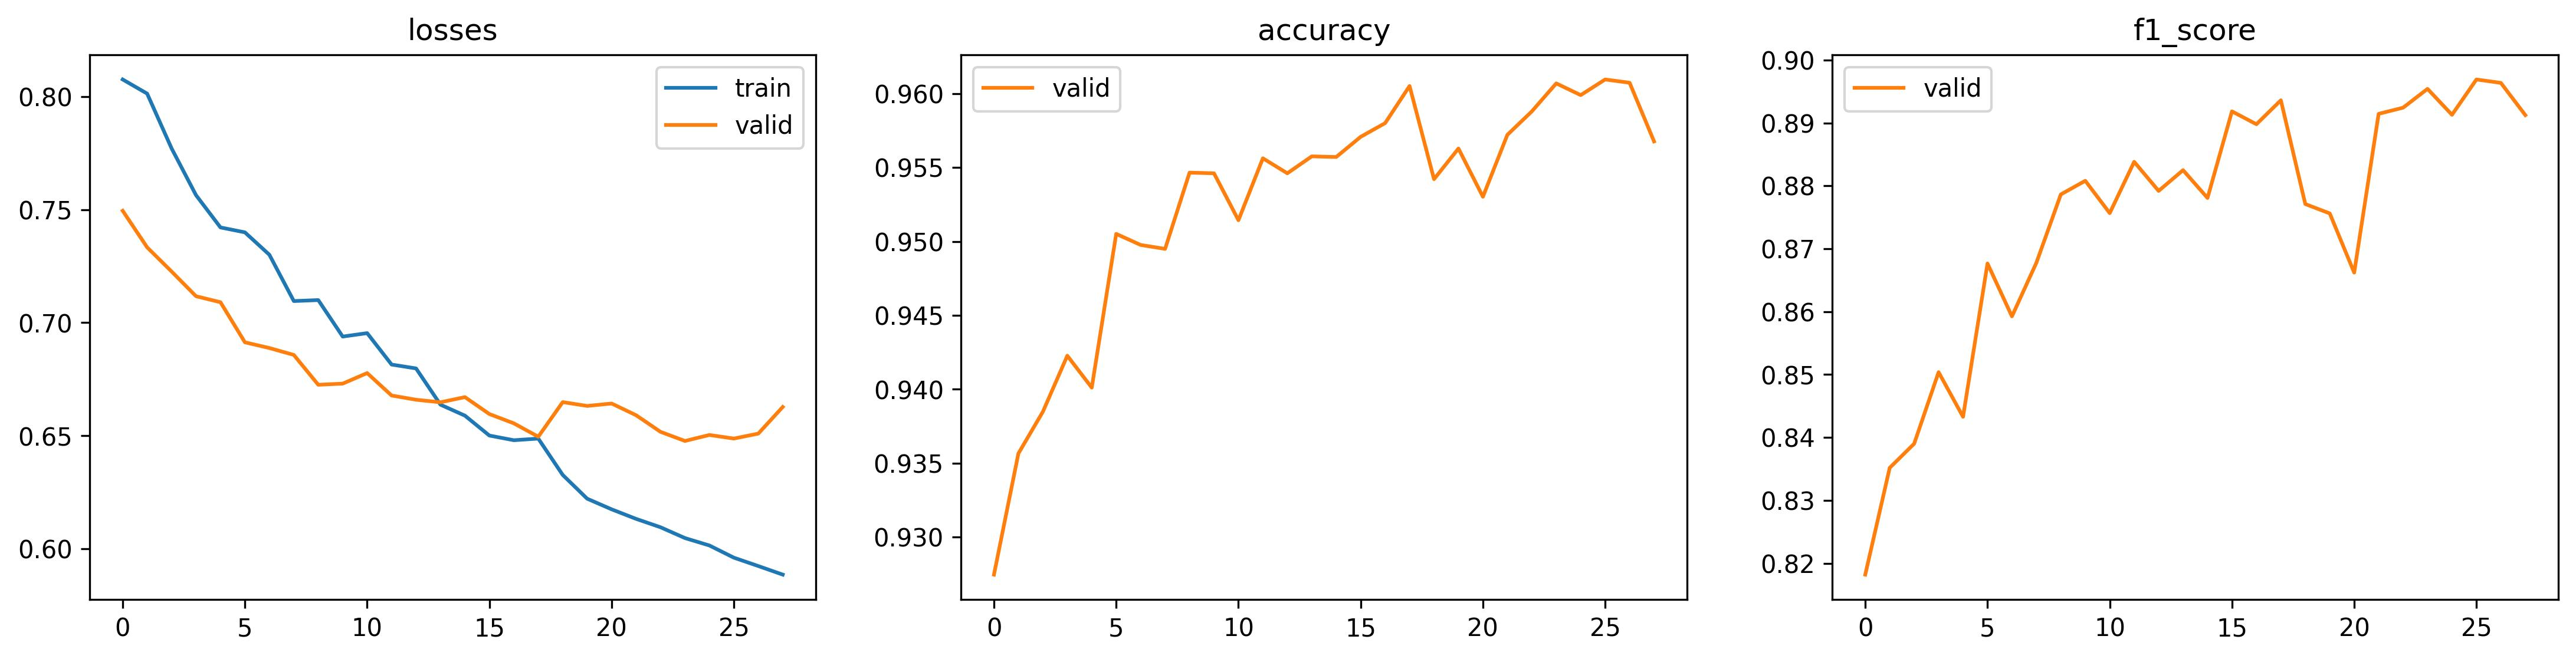
\includegraphics[width=\textwidth]{img/cap09/curvas_vit_base_patch16_224.jpg}
%  \caption{ViT-B/16 (\texttt{vit\_base\_patch16\_224}): curvas de entrenamiento.}
%  \label{fig:curvas-vit}
%\end{figure}

%\begin{figure}[tbp]
%  \centering
%  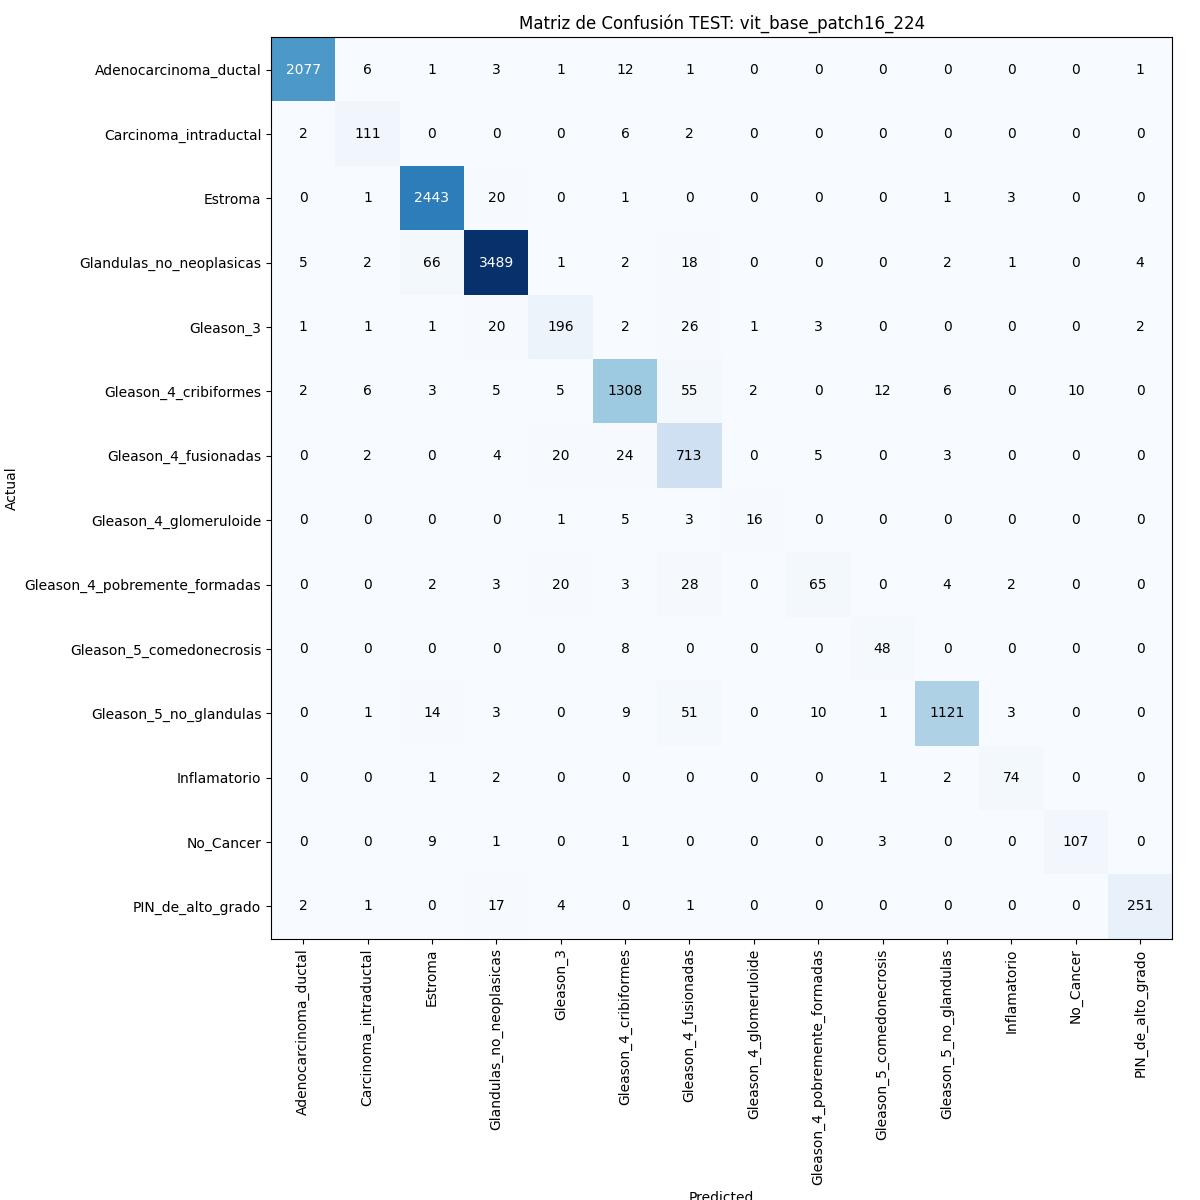
\includegraphics[width=\textwidth]{img/cap09/confusion_test_vit_base_patch16_224.jpg}
%  \caption{ViT-B/16 (\texttt{vit\_base\_patch16\_224}): matriz de confusión en el test.}
%  \label{fig:confusion-vit}
%\end{figure}

Pérdida en test: 0,8892; exactitud en test: 0,8964.
%\revisar{las notas daban 0,8963 (\texttt{resultados.txt}); se usa el valor de results\_fase1}
\pendiente{análisis}

%\begin{figure}[tbp]
%  \centering
%  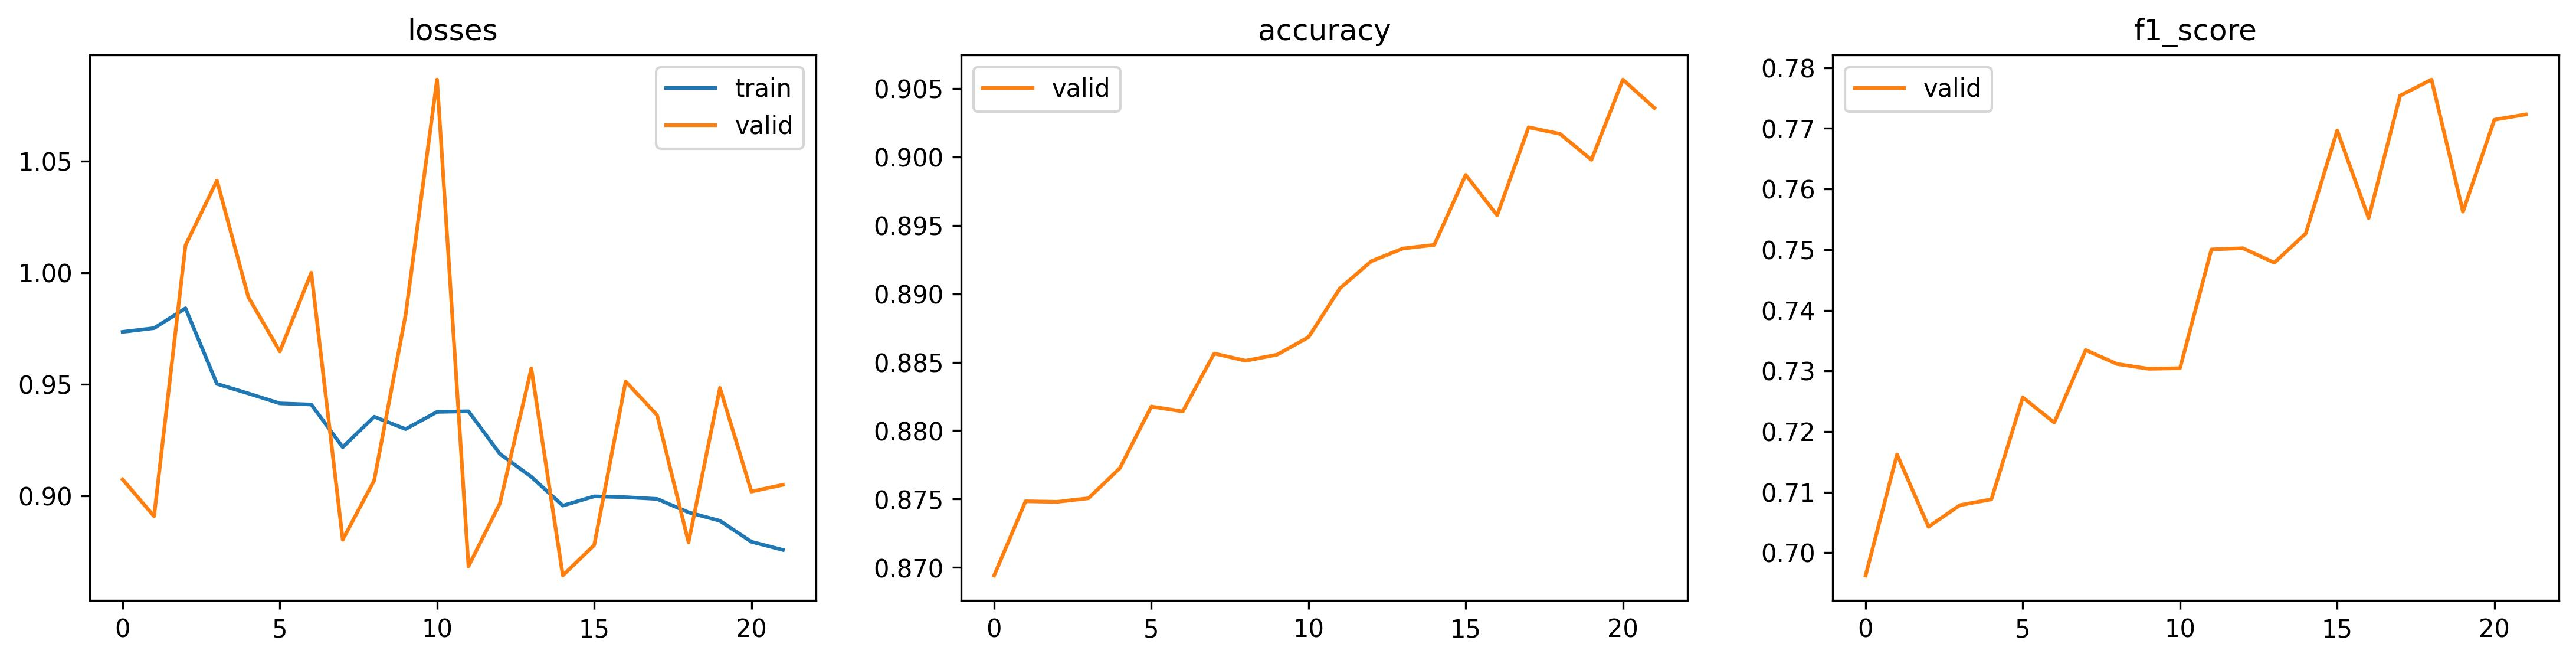
\includegraphics[width=\textwidth]{img/cap09/curvas_resnet50.jpg}
%  \caption{ResNet-50 (\texttt{resnet50}): curvas de entrenamiento.}
%  \label{fig:curvas-resnet}
%\end{figure}

%\begin{figure}[tbp]
%  \centering
%  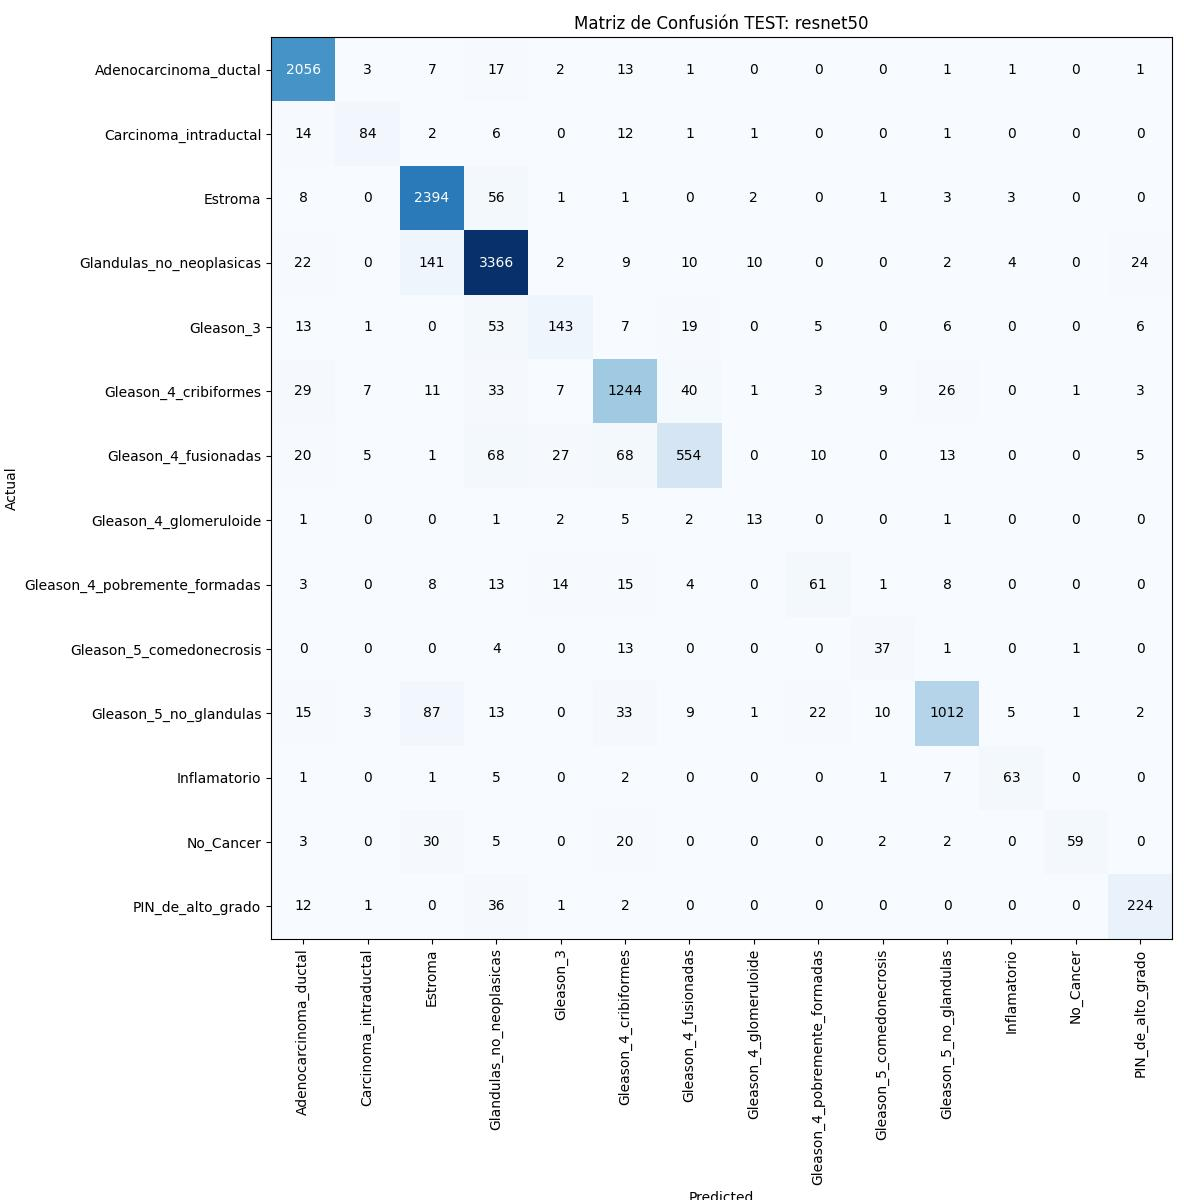
\includegraphics[width=\textwidth]{img/cap09/confusion_test_resnet50.jpg}
%  \caption{ResNet-50 (\texttt{resnet50}): matriz de confusión en el test.}
%  \label{fig:confusion-resnet}
%\end{figure}

Pérdida en test: 0,6424; exactitud en test: 0,9668.
\pendiente{análisis}

%\begin{figure}[tbp]
%  \centering
%  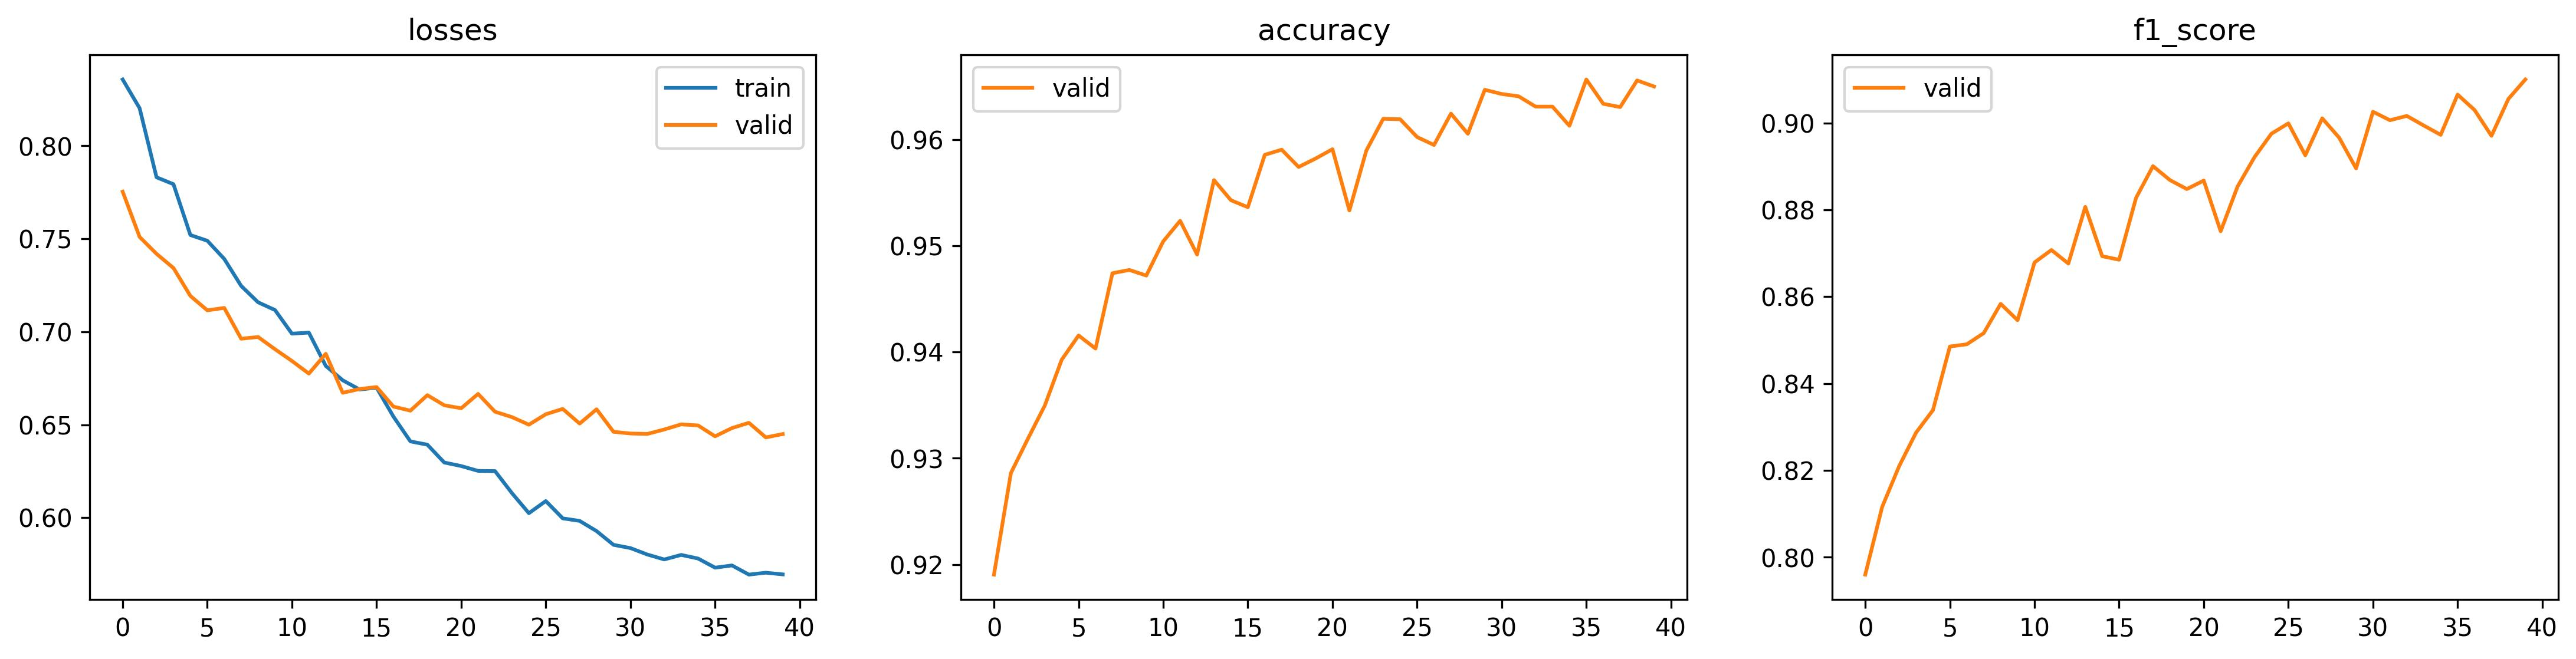
\includegraphics[width=\textwidth]{img/cap09/curvas_convnext_small.jpg}
%  \caption{ConvNeXt-S (\texttt{convnext\_small}, entrenado y evaluado a 256\,px): curvas de entrenamiento.}
%  \label{fig:curvas-convnext}
%\end{figure}

%\begin{figure}[tbp]
%  \centering
%  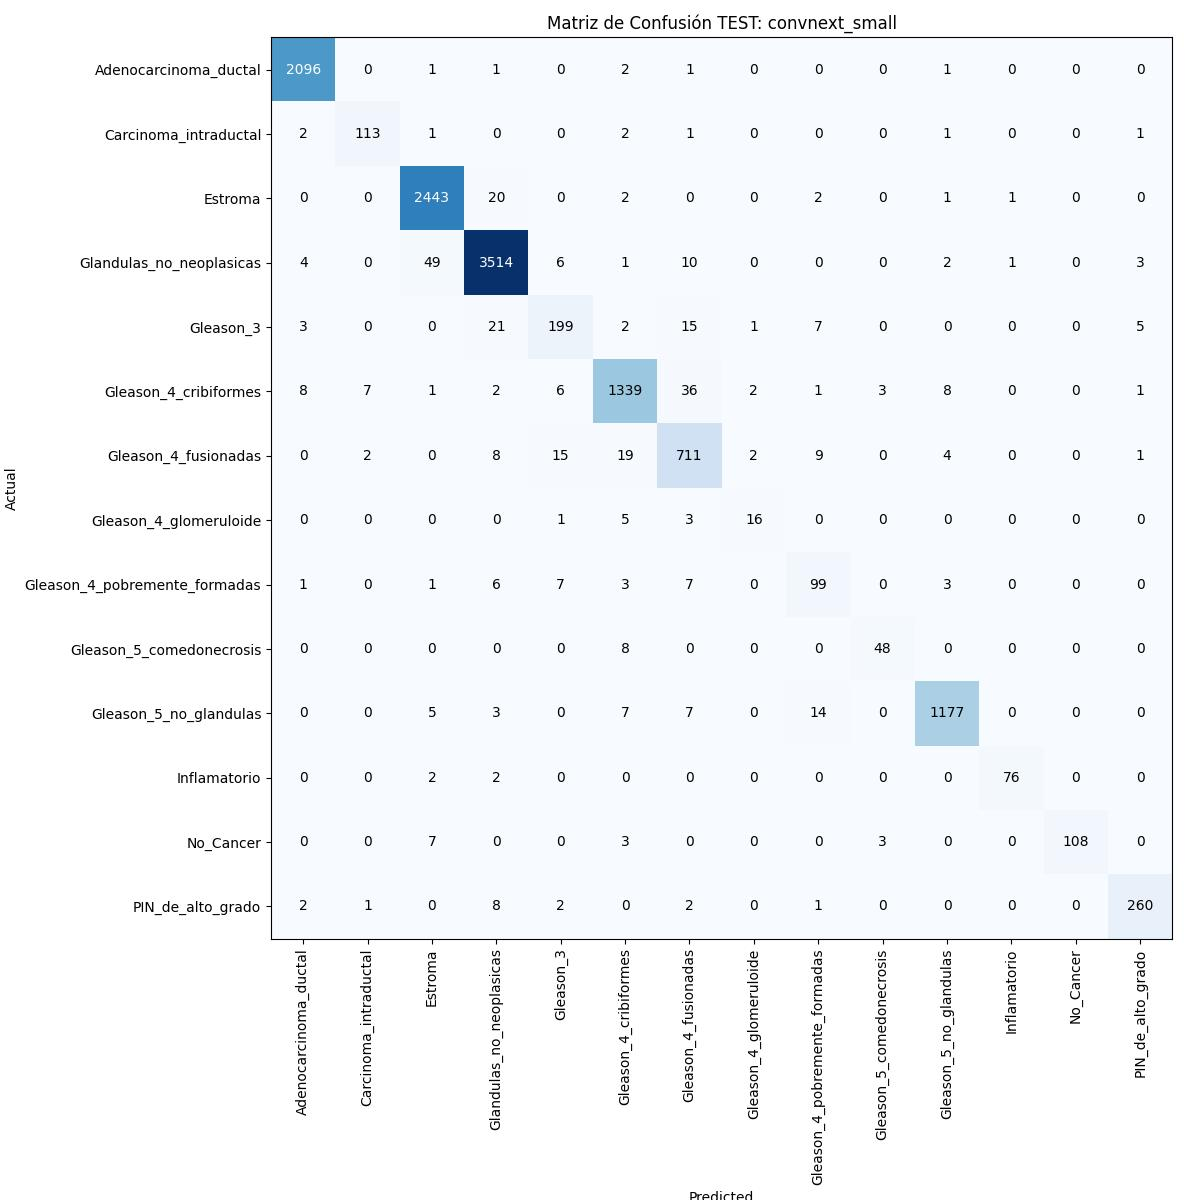
\includegraphics[width=\textwidth]{img/cap09/confusion_test_convnext_small.jpg}
%  \caption{ConvNeXt-S (\texttt{convnext\_small}, entrenado y evaluado a 256\,px): matriz de confusión en el test.}
%  \label{fig:confusion-convnext}
%\end{figure}

% Las notas no daban la pérdida ni la exactitud de este modelo («Modelo 4»); valores de
% resultados.txt (param3): pérdida 0,6757; exactitud 0,9538.
\pendiente{análisis (pérdida en test: 0,6757; exactitud en test: 0,9538)}

%\begin{figure}[tbp]
%  \centering
%  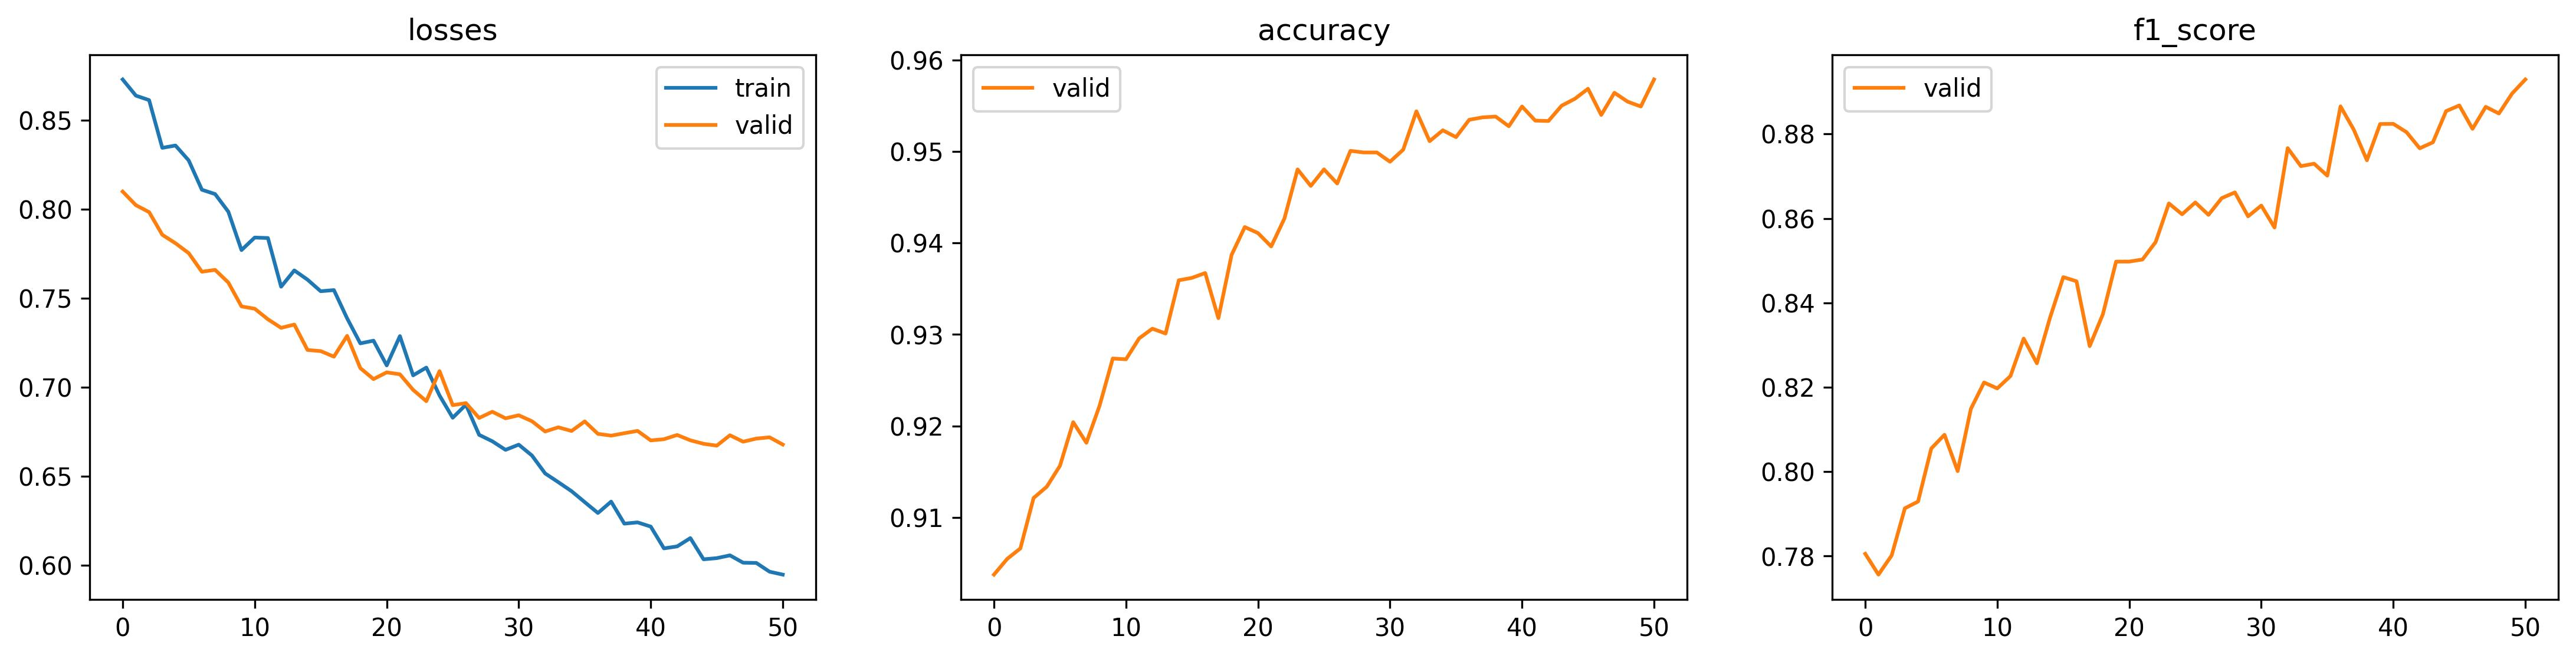
\includegraphics[width=\textwidth]{img/cap09/curvas_tf_efficientnetv2_s.jpg}
%  \caption{EfficientNetV2-S (\texttt{tf\_efficientnetv2\_s}): curvas de entrenamiento.}
%  \label{fig:curvas-efficientnet}
%\end{figure}

%\begin{figure}[tbp]
%  \centering
%  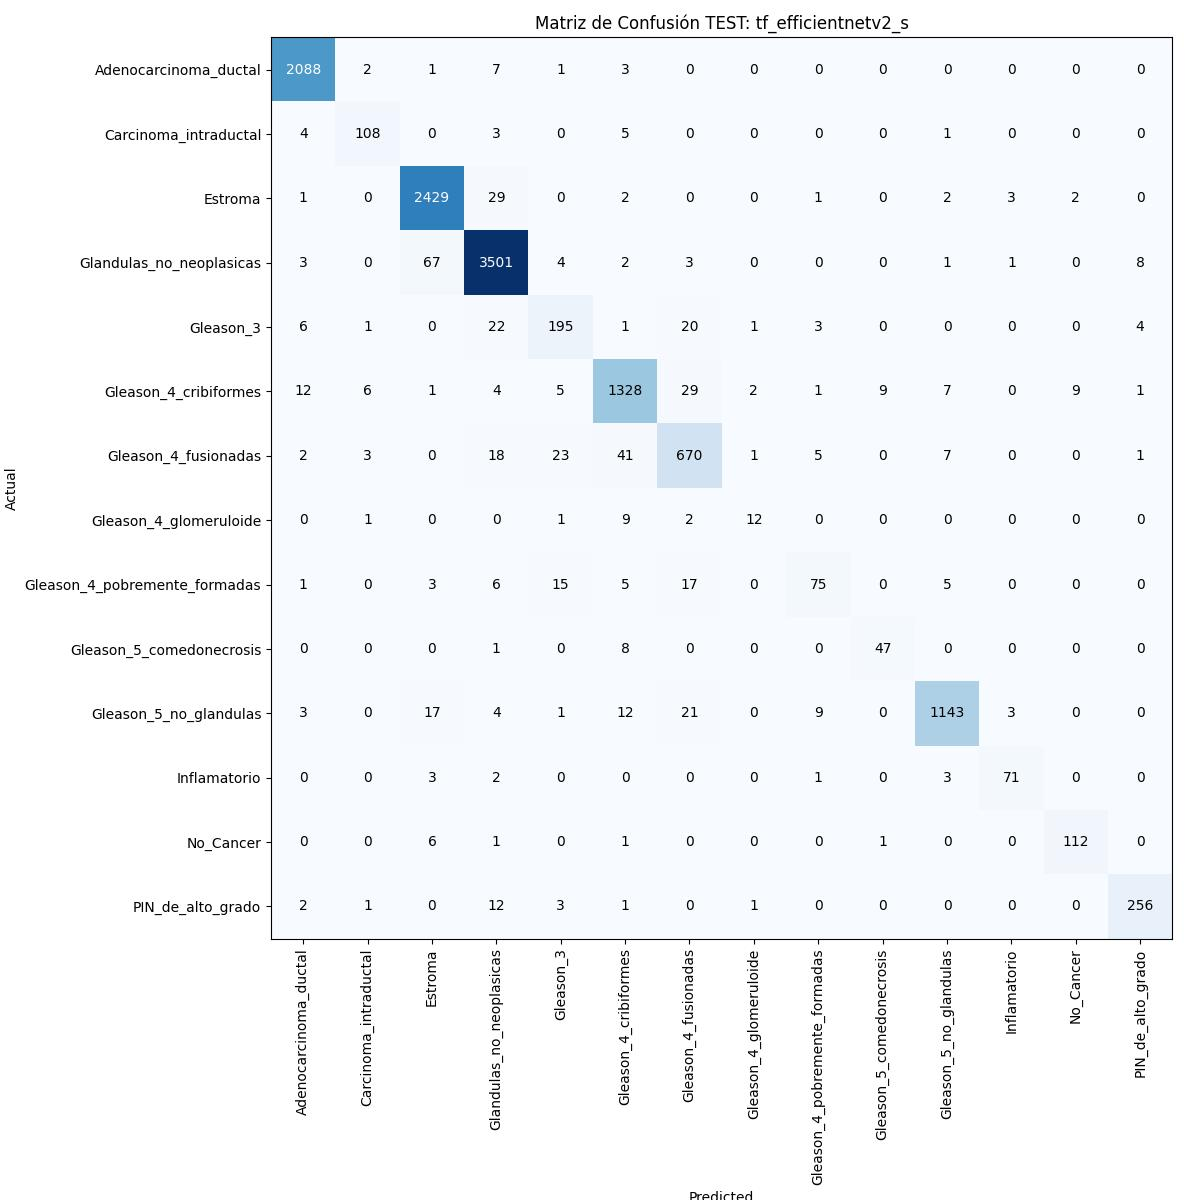
\includegraphics[width=\textwidth]{img/cap09/confusion_test_tf_efficientnetv2_s.jpg}
%  \caption{EfficientNetV2-S (\texttt{tf\_efficientnetv2\_s}): matriz de confusión en el test.}
%  \label{fig:confusion-efficientnet}
%\end{figure}

% Las gráficas del Swin faltaban en las notas. resultados.txt (param4): pérdida en test 0,6356;
% entrenamiento de 583,6 min en una TITAN Xp. Confusiones más frecuentes: Glándulas no
% neoplásicas -> Estroma (62), Gleason_4_cribiformes -> Gleason_4_fusionadas (57), Estroma ->
% Glándulas no neoplásicas (47), Gleason_4_fusionadas -> Gleason_4_cribiformes (41).
\pendiente{análisis (pérdida en test: 0,6356; exactitud en test: 0,9688)}

\begin{figure}[tbp]
  \centering
  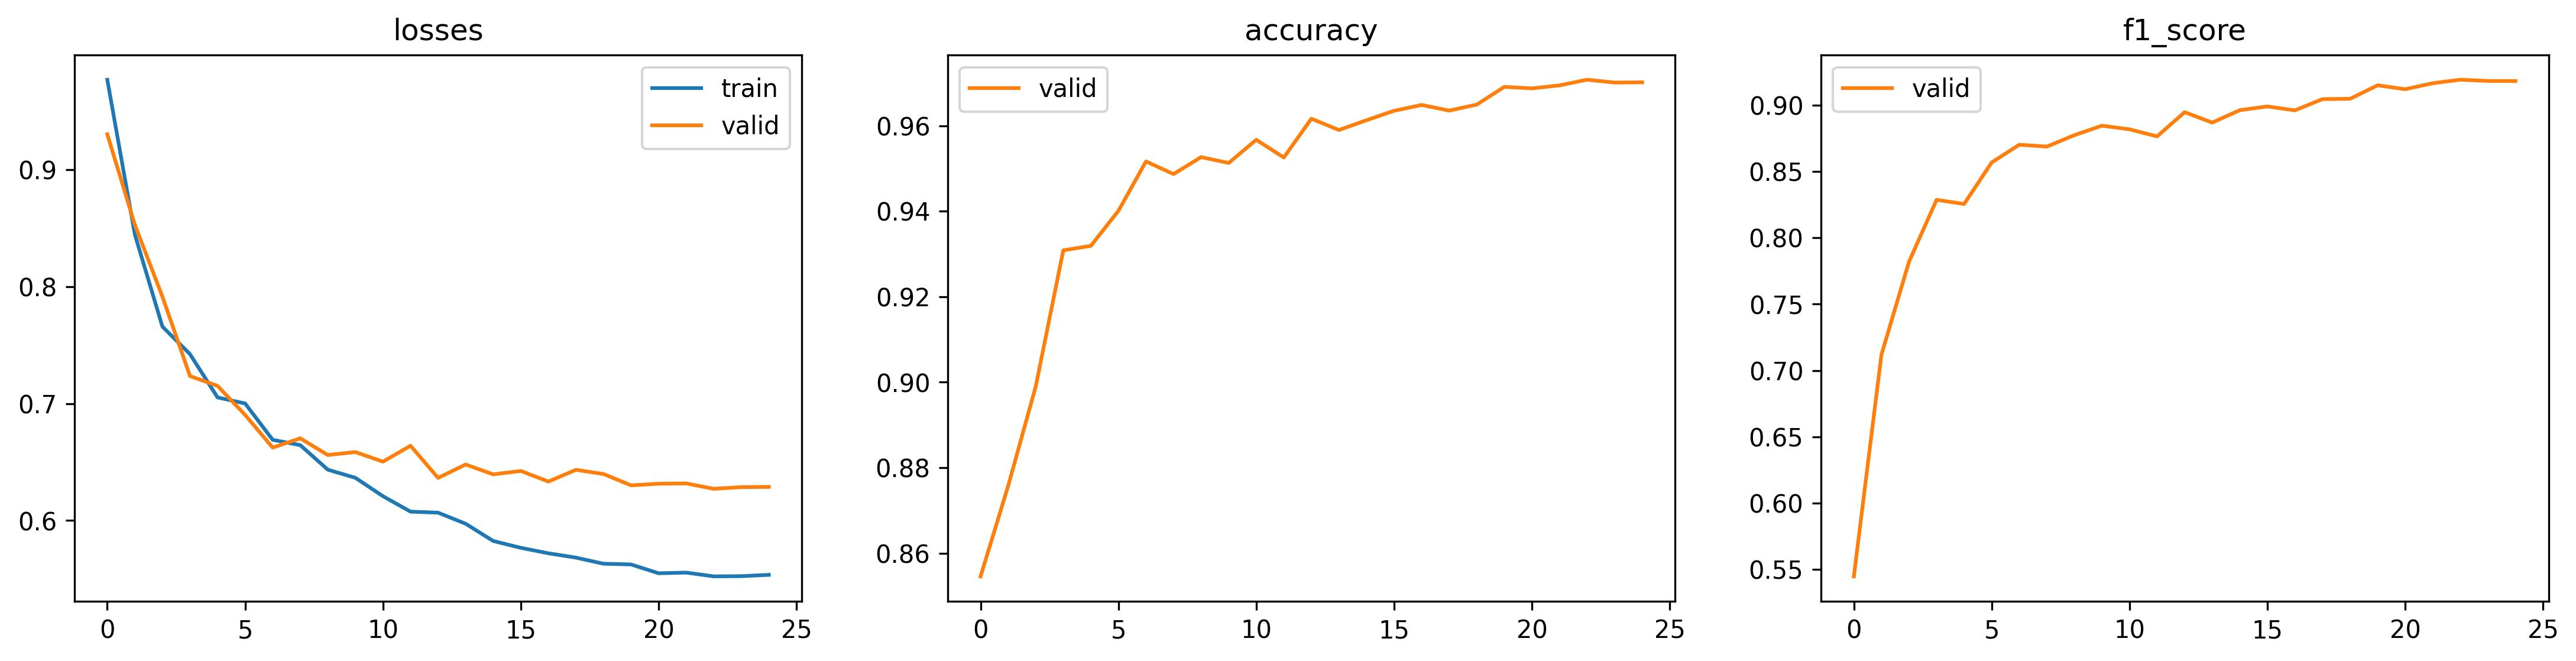
\includegraphics[width=\textwidth]{img/cap09/curvas_swin_small_patch4_window7_224.jpg}
  \caption{Swin-S (\texttt{swin\_small\_patch4\_window7\_224}): curvas de entrenamiento.}
  \label{fig:curvas-swin}
\end{figure}

\begin{figure}[tbp]
  \centering
  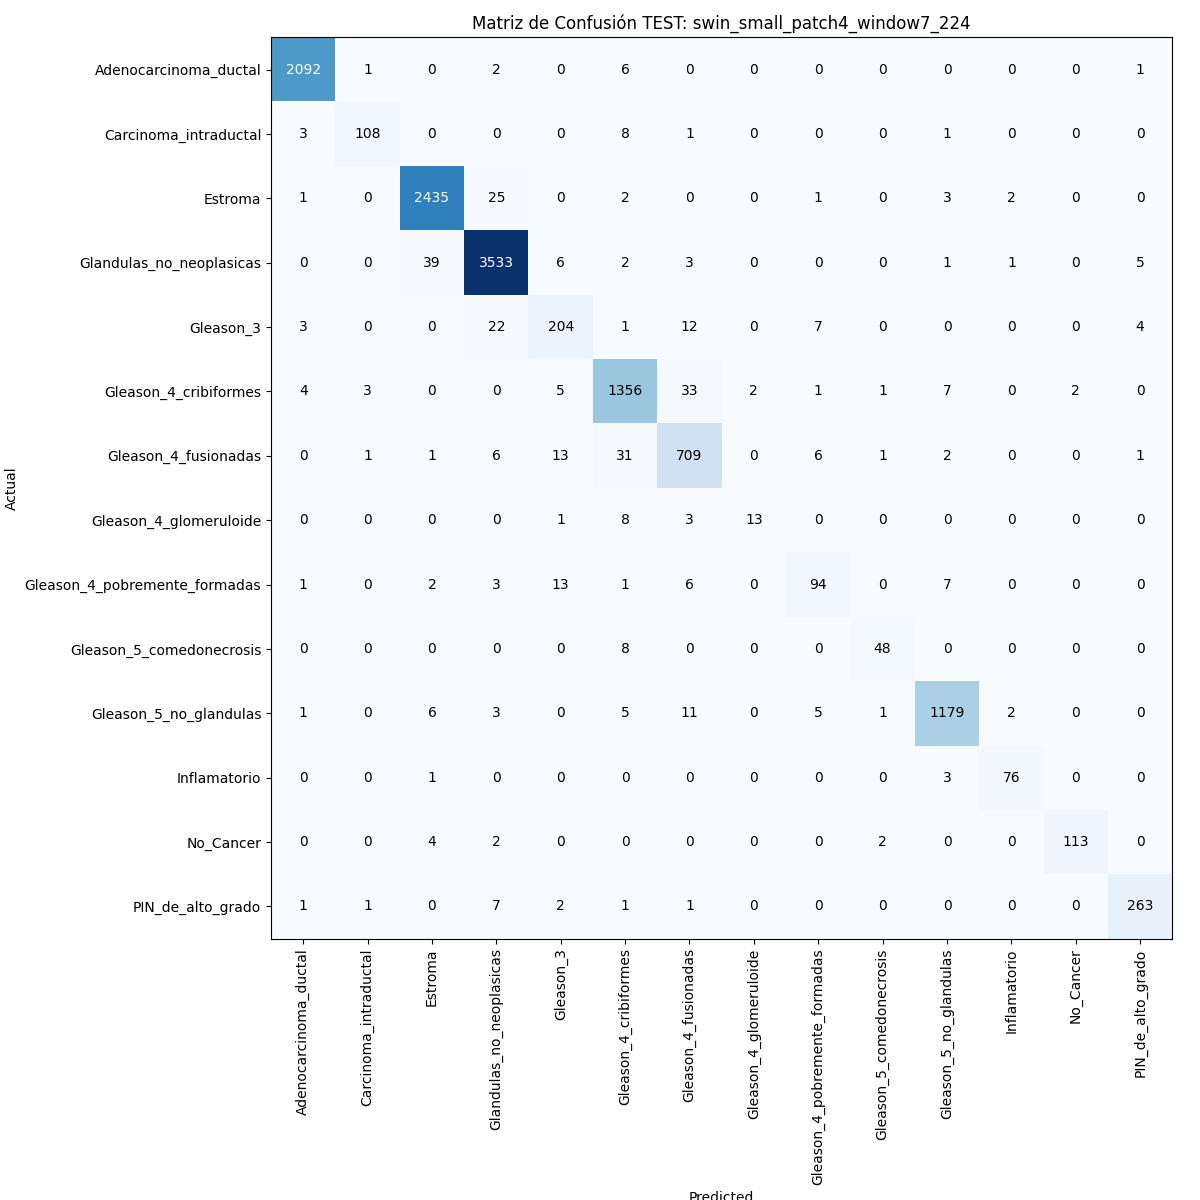
\includegraphics[width=\textwidth]{img/cap09/confusion_test_swin_small_patch4_window7_224.jpg}
  \caption{Swin-S (\texttt{swin\_small\_patch4\_window7\_224}): matriz de confusión en el test.}
  \label{fig:confusion-swin}
\end{figure}


\subsection{Sensibilidad por clase}\label{sec:modelos-recall}

% Cifras clave (results_fase1): las cinco arquitecturas fallan en las mismas clases minoritarias.
% Gleason_4_glomeruloide (25 imágenes): 0,52 (Swin), 0,64 (ConvNeXt), 0,48, 0,64 y 0,52;
% Gleason_4_pobremente_formadas (127): 0,74, 0,78, 0,59, 0,51 y 0,48; Gleason_3 (253): 0,81, 0,79,
% 0,77, 0,78 y 0,57 (orden: Swin, ConvNeXt, EfficientNetV2, ViT, ResNet). Swin supera a ConvNeXt en
% Gleason_3, cribiformes, No_Cancer y PIN; ConvNeXt a Swin en Carcinoma_intraductal, glomeruloide y
% pobremente formadas.
% Márgenes de Swin-S cuando gana (recall_por_clase.csv): Gleason_3 +0,0198, cribiformes +0,0120,
% PIN +0,0109, No_Cancer +0,0083, Glandulas_no_neoplasicas +0,0056, Gleason_5_no_glandulas +0,0016;
% empates: Inflamatorio y Gleason_5_comedonecrosis. Diferencia < 0,01: Estroma, Adenocarcinoma_ductal,
% Gleason_4_fusionadas. Gleason_3: 2.275 imágenes de train+val frente a 6.938 de Gleason_4_fusionadas.
Se puede observar que Swin-S gana o empata en 8 clases y en otras 3 la diferencia es inferior a $10^{-2}$ (\cref{tab:recall-clase}). Aunque en aquellos casos en los que gana la diferencia no es en ningún caso mayor que $2 \cdot 10^{-2}$, puede considerarse un argumento a favor de su elección, si bien no concluyente. Por otro lado, simplemente observando la \cref{tab:recall-clase}, se aprecia cómo 4 clases no alcanzan en ningún modelo el valor 0,90 de \emph{recall}. A continuación se muestra cuáles son esas clases y los posibles motivos de lo ocurrido:
\begin{itemize}
  \item \textbf{Gleason 3:} como se vio en la \cref{sec:conjunto-id}, los modelos confunden Gleason 3 con Gleason 4 fusionadas y viceversa. ¿Por qué, si esta confusión ocurre en los dos sentidos, la clase Gleason 4 fusionadas presenta una mayor sensibilidad? Esto puede deberse a que Gleason 3 presenta una cantidad de muestras tres veces menor (\cref{tab:particion}), lo que hace que los modelos generalicen peor para Gleason 3.
  \item \textbf{Gleason 4 pobremente formadas:} como se vio en la \cref{tab:clases}, esta clase presenta una definición muy pobre, por lo que es entendible que al modelo le cueste sacar patrones o relaciones entre imágenes entre las cuales existe poca relación.
  \item \textbf{Gleason 5 comedonecrosis:} igualmente, esta cuestión se discutió en la \cref{sec:conjunto-id}, y es que los modelos presentan una fuerte tendencia a confundir las muestras de Gleason 5 comedonecrosis con Gleason 4 cribiformes debido a la estructura similar que presentan.
  \item \textbf{Gleason 4 glomeruloide:} como se puede apreciar en la \cref{tab:particion}, se trata de la clase con menor conjunto de muestras y, al no presentar características fuertemente definitorias, al modelo le resulta muy complicado abstraerla, generando así los resultados más bajos de \emph{recall} de toda la \cref{tab:recall-clase}.
\end{itemize}

% Generado por scripts/generar_tablas.py a partir de results_fase1/recall_por_clase.csv. No editar a mano.
\begin{table}
\centering
\scriptsize
\setlength{\tabcolsep}{4pt}
\caption{Sensibilidad (\emph{recall}) por clase en el test ID de los cinco modelos (más alto es mejor); $n$: imágenes de test de la clase. En negrita, el mejor valor de cada clase.}
\label{tab:recall-clase}
\begin{tabular}{lrccccc}
\toprule
Clase & $n$ & Swin-S & ConvNeXt-S & EfficientNetV2-S & ViT-B/16 & ResNet-50 \\
\midrule
\clase{Glandulas\_no\_neoplasicas} & \num{3590} & \textbf{0{,}98} & 0{,}98 & 0{,}98 & 0{,}97 & 0{,}94 \\
\clase{Estroma} & \num{2469} & 0{,}99 & \textbf{0{,}99} & 0{,}98 & \textbf{0{,}99} & 0{,}97 \\
\clase{Adenocarcinoma\_ductal} & \num{2102} & 1{,}00 & \textbf{1{,}00} & 0{,}99 & 0{,}99 & 0{,}98 \\
\clase{Gleason\_4\_cribiformes} & \num{1414} & \textbf{0{,}96} & 0{,}95 & 0{,}94 & 0{,}93 & 0{,}88 \\
\clase{Gleason\_5\_no\_glandulas} & \num{1213} & \textbf{0{,}97} & 0{,}97 & 0{,}94 & 0{,}92 & 0{,}83 \\
\clase{Gleason\_4\_fusionadas} & \num{771} & 0{,}92 & 0{,}92 & 0{,}87 & \textbf{0{,}92} & 0{,}72 \\
\clase{PIN\_de\_alto\_grado} & \num{276} & \textbf{0{,}95} & 0{,}94 & 0{,}93 & 0{,}91 & 0{,}81 \\
\clase{Gleason\_3} & \num{253} & \textbf{0{,}81} & 0{,}79 & 0{,}77 & 0{,}77 & 0{,}57 \\
\clase{Gleason\_4\_pobremente\_formadas} & \num{127} & 0{,}74 & \textbf{0{,}78} & 0{,}59 & 0{,}51 & 0{,}48 \\
\clase{Carcinoma\_intraductal} & \num{121} & 0{,}89 & \textbf{0{,}93} & 0{,}89 & 0{,}92 & 0{,}69 \\
\clase{No\_Cancer} & \num{121} & \textbf{0{,}93} & 0{,}89 & 0{,}93 & 0{,}88 & 0{,}49 \\
\clase{Inflamatorio} & \num{80} & \textbf{0{,}95} & \textbf{0{,}95} & 0{,}89 & 0{,}93 & 0{,}79 \\
\clase{Gleason\_5\_comedonecrosis} & \num{56} & \textbf{0{,}86} & \textbf{0{,}86} & 0{,}84 & \textbf{0{,}86} & 0{,}66 \\
\clase{Gleason\_4\_glomeruloide} & \num{25} & 0{,}52 & \textbf{0{,}64} & 0{,}48 & \textbf{0{,}64} & 0{,}52 \\
\bottomrule
\end{tabular}
\end{table}



\section{Elección del modelo}\label{sec:eleccion-swin}

El modelo Swin Transformer obtiene la mayor exactitud (96,88\,\%), seguido muy de cerca por ConvNeXt (96,68\,\%). Dada la escasa diferencia entre ambos, cualquiera de los dos sería una base adecuada; se selecciona Swin por ser el que mejor resultado ha obtenido, aunque como ya se ha visto no se puede asegurar que sea el mejor modelo con certeza.

\revisar{exactitud del Swin-S: 96,87\,\% en las notas, 96,88\,\% en results\_fase1 (valor único de la memoria)}
\revisar{la diferencia no es estadísticamente significativa (McNemar $p = 0{,}19$, \cref{tab:mcnemar}; ConvNeXt-S tiene además mayor F1 macro y \emph{balanced accuracy}): la elección no puede justificarse por un mejor resultado, sino presentarse como elección entre dos modelos empatados}

% Generado por scripts/generar_tablas.py a partir de results_fase1/swin_vs_convnext.json. No editar a mano.
\begin{table}
\centering
\small
\caption{Tabla de contingencia de aciertos de Swin-S y ConvNeXt-S sobre las mismas 12.618 imágenes de test. Test de McNemar: $p$ exacto (binomial) $= 0{,}188$; $\chi^2$ con corrección de continuidad $= 1{,}73$ ($p = 0{,}188$). \emph{Bootstrap} pareado de la diferencia de exactitud Swin-S $-$ ConvNeXt-S: $+0{,}0020$ [-0{,}0011; 0{,}0049] ($p = 0{,}18$; por lámina [-0{,}0013; 0{,}0049], $p = 0{,}24$); de F1 macro: $-0{,}0004$ [-0{,}0135; 0{,}0107] ($p = 0{,}98$).}
\label{tab:mcnemar}
\begin{tabular}{lcc}
\toprule
& ConvNeXt-S acierta & ConvNeXt-S falla \\
\midrule
Swin-S acierta & \num{12045} & \num{179} \\
Swin-S falla & \num{154} & \num{240} \\
\bottomrule
\end{tabular}
\end{table}


La superioridad de esta arquitectura radica en tres pilares fundamentales:

\begin{enumerate}
  \item \textbf{Jerarquización y ventanas desplazadas (\emph{shifted windows}).} A diferencia de los Vision Transformers (ViT) estándar, que operan con parches globales, el Swin Transformer utiliza un mecanismo de ventanas jerárquicas~\cite[sec.~1 y fig.~1]{liu2021swin}. Esto permite capturar relaciones espaciales tanto a nivel local (textura, morfología de tejidos) como global (anatomía estructural de la lesión).
  \item \textbf{Eficiencia en el contexto local.} La capacidad de contextualizar parches mediante ventanas de $7 \times 7$ (\texttt{window7})~\cite[sec.~3.2]{liu2021swin} permite que el modelo se enfoque en características relevantes sin verse afectado por el ruido de fondo, algo que los modelos de atención global (como \texttt{vit\_base\_patch16}) pueden ignorar al tratar todas las regiones por igual. \revisar{«mediante window7» se ha desarrollado como «mediante ventanas de $7 \times 7$ (\texttt{window7})»}
  \item \textbf{Inductividad de la imagen.} Al igual que ConvNeXt, el Swin Transformer integra principios de las redes convolucionales (sesgo inductivo)~\cite[sec.~4.4]{liu2021swin}, lo que facilita el aprendizaje de características jerárquicas desde resoluciones finas a gruesas. Esto permite una convergencia más eficiente y un mejor aprovechamiento de la información contenida en las imágenes médicas.
\end{enumerate}

\begin{itemize}
  \item \textbf{Complementariedad de enfoques.} El hecho de que modelos basados en atención jerárquica y arquitecturas convolucionales modernas compitan por el primer puesto sugiere que las características más relevantes para el diagnóstico están siendo bien capturadas por ambos paradigmas.
\end{itemize}

A pesar de que Swin-S sea el modelo que ha dado mejores resultados cabe preguntarse si esto realmente puede llegar a ser suficiente como para considerarlo mejor 
que el segundo mejor modelo, ConvNeXt, habiendo sido ambos evaluados sobre las mismas \num{12618} imágenes del test ID. Para resolver esta cuestión se va a emplear el test de McNemar, siguiendo la teoría descrita en la \cref{sec:mcnemar}.

\begin{table}[H]
  \centering
  \caption{Tabla de contingencia del test de McNemar entre Swin-S y ConvNeXt-S sobre las \num{12618} imágenes del test ID. En negrita, los pares discordantes.}
  \label{tab:mcnemar-swin-convnext}
  \begin{tabular}{lcc}
    \toprule
    & ConvNeXt-S acierta & ConvNeXt-S falla \\
    \midrule
    Swin-S acierta & \num{12045} & \textbf{179} \\
    Swin-S falla   & \textbf{154} & 240 \\
    \bottomrule
  \end{tabular}
\end{table}

Denotamos por $a$ el número de imágenes en las que ambos aciertan (\num{12045}), por $b$ aquellas en las que solo acierta Swin-S (179), por $c$ aquellas en las que solo acierta ConvNeXt-S (154) y por $d$ aquellas en las que ambos fallan (240).

\textbf{Hipótesis:}
\begin{itemize}
  \item $H_0$: ambos modelos presentan la misma capacidad de acierto. Cuando discrepan, cada uno tiene una probabilidad de $\tfrac{1}{2}$ de ser el que acierta.
  \item $H_1$: dicha probabilidad es distinta de $\tfrac{1}{2}$.
\end{itemize}

Bajo $H_0$, y condicionando al número de pares discordantes, $n = b + c = 179 + 154 = 333$, el número de pares favorables a Swin-S sigue una distribución binomial (\cref{prop:mcnemar}):
\[
  b \sim \mathrm{Bin}\left(333, \tfrac{1}{2}\right), \qquad
  \E[b] = \frac{333}{2} = 166{,}5, \qquad
  \Var(b) = 333 \cdot \frac{1}{2}\left(1 - \frac{1}{2}\right) = 83{,}25.
\]

% --- CONTINUACIÓN (nuevo) ---
\textbf{Versión exacta.} El $p$-valor bilateral es la probabilidad, bajo $H_0$, de obtener un reparto al menos tan desequilibrado como el observado:
\[
  p = 2\,\Prob(X \geq 179) = 0{,}188, \qquad X \sim \mathrm{Bin}\left(333, \tfrac{1}{2}\right).
\]
% --- FIN DE LA CONTINUACIÓN; sigue tu texto ---

\textbf{Aproximación normal.} Una binomial es una suma de $n$ variables de Bernoulli independientes. Por el teorema central del límite, que en el caso de la binomial es el teorema de De Moivre-Laplace~\cite{canavos2003}, para un valor de $n$ lo suficientemente grande es aproximadamente normal. Tipificando se tiene:
\[
  Z = \frac{b - n/2}{\sqrt{n/4}} \;\overset{\text{aprox.}}{\sim}\; N(0, 1).
\]
Sustituyendo $n = b + c$, se tiene $b - \frac{n}{2} = \frac{b - c}{2}$ y $\sqrt{n/4} = \frac{\sqrt{b + c}}{2}$, de modo que
\[
  Z = \frac{b - c}{\sqrt{b + c}} = \frac{179 - 154}{\sqrt{333}} = \frac{25}{18{,}248} = 1{,}370.
\]
Al trabajar con la normal, que es continua, se obtiene un resultado más aproximado aplicando la corrección de continuidad, debido a la naturaleza discreta de los datos:
\[
  Z_c = \frac{|b - c| - 1}{\sqrt{b + c}} = \frac{24}{18{,}248} = 1{,}315.
\]


El $p$-valor bilateral es entonces
\[
  p = 2\left(1 - \Phi(1{,}315)\right) = 2 \cdot 0{,}0942 = 0{,}188,
\]
que coincide con el exacto. Sin la corrección se obtendría $p = 0{,}171$, que subestima el $p$-valor. Equivalentemente, $\chi^2_c = Z_c^2 = 1{,}730$ sigue aproximadamente una distribución $\chi^2_1$, y $\Prob(\chi^2_1 \geq 1{,}730) = 0{,}188$.

\textbf{Decisión.} Con un nivel de significación $\alpha = 0{,}05$, como $p = 0{,}188 > \alpha$, no se rechaza la hipótesis nula: no hay evidencia de que Swin-S y ConvNeXt-S difieran en exactitud. Para rechazarla, la región crítica $\chi^2_c > \chi^2_{1;\,0{,}95} = 3{,}841$ exigiría $|b - c| \geq 37$. Un caso podría ser por ejemplo que Swin-S ganara 185 de los 333 pares discordantes en lugar de 179.

\textbf{Diferencia observada.} Con la notación de la \cref{tab:mcnemar-swin-convnext} y $N = a + b + c + d = \num{12618}$, la exactitud de Swin-S es $(a + b)/N$ y la de ConvNeXt-S, $(a + c)/N$. Los aciertos comunes se cancelan y la diferencia solo depende de los pares discordantes:
\[
  \hat\Delta = \frac{a + b}{N} - \frac{a + c}{N} = \frac{b - c}{N} = \frac{179 - 154}{\num{12618}} = \frac{25}{\num{12618}} = 0{,}00198 \approx +0{,}0020.
\]

\textbf{Limitación.} El test supone que los pares discordantes son independientes. Esta hipótesis no se cumple del todo, porque las imágenes de una misma lámina están relacionadas (\cref{cap:fuga}). Por ello, para constratar este resultado se realizará un \emph{bootstrap} pareado por lámina (\cref{sec:bootstrap}):

\textbf{\emph{Bootstrap} pareado por lámina.} Se aplica el procedimiento del \cref{sec:bootstrap} con dos particularidades (\cref{obs:bootstrap-variantes}): la unidad que se remuestrea es la lámina, no la imagen, y las dos exactitudes se calculan sobre la misma muestra remuestreada. Sean $L$ las láminas del test ID e $I_\ell$ el conjunto de imágenes de la lámina $\ell$. Para un multiconjunto de índices $J$, la exactitud del modelo $m$ es
\[
  \mathrm{Acc}_m(J) = \frac{1}{|J|} \sum_{i \in J} \Ind\bigl(\hat y^{(m)}_i = y_i\bigr),
\]
donde $\Ind(\cdot)$ es la función indicadora (\cref{sec:bootstrap}), $\hat y^{(m)}_i$ es la predicción del modelo $m$ para la imagen $i$ e $y_i$, su clase real.
En cada réplica $b = 1, \dots, B$:
\begin{enumerate}
  \item Se eligen $L$ láminas con reemplazo, $\ell^{*}_{1}, \dots, \ell^{*}_{L} \overset{\text{i.i.d.}}{\sim} \mathcal{U}\{1, \dots, L\}$, y se toman todas sus imágenes, $J^{*}_{b} = I_{\ell^{*}_{1}} \cup \dots \cup I_{\ell^{*}_{L}}$ (con repeticiones). El número de imágenes $|J^{*}_{b}|$ varía de una réplica a otra.
  \item Se calcula la diferencia sobre esas imágenes, con los mismos índices para los dos modelos:
  \[
    \Delta^{*}_{b} = \mathrm{Acc}_{\text{Swin}}\bigl(J^{*}_{b}\bigr) - \mathrm{Acc}_{\text{ConvNeXt}}\bigl(J^{*}_{b}\bigr).
  \]
\end{enumerate}
Con $B = \num{1000}$ réplicas (semilla 0), el intervalo de confianza del 95\,\% por percentiles (\cref{def:bootstrap}) lo forman los percentiles 2,5 y 97,5 de $\Delta^{*}_{1}, \dots, \Delta^{*}_{B}$, calculados con interpolación lineal entre las dos réplicas ordenadas más próximas:
\[
  \text{IC}_{\text{95\,\%}}(\Delta) = [-0{,}0013;\ +0{,}0049].
\]

El intervalo contiene el cero, por lo que la diferencia no es significativa. Para obtener un $p$-valor \emph{bootstrap} bilateral se cuenta qué proporción de réplicas queda a cada lado del cero,
\[
  \hat\pi_{\le} = \frac{1}{B} \sum_{b=1}^{B} \Ind\bigl(\Delta^{*}_{b} \le 0\bigr), \qquad
  \hat\pi_{\ge} = \frac{1}{B} \sum_{b=1}^{B} \Ind\bigl(\Delta^{*}_{b} \ge 0\bigr),
\]
y se toma el doble de la menor, por ser un contraste bilateral, sin superar 1:
\[
  p^{*} = \min\bigl\{1,\ 2 \min\bigl(\hat\pi_{\le},\ \hat\pi_{\ge}\bigr)\bigr\} = 0{,}244.
\]
Con esta definición, $p^{*} < \alpha$ equivale, salvo por la interpolación de los percentiles, a que el cero quede fuera del intervalo por percentiles de nivel $1 - \alpha$~\cite{pena2008fundamentos}; por eso el $p$-valor y el intervalo llevan a la misma decisión. Este resultado conduce a la misma conclusión que el test de McNemar ($p = 0{,}188$). Si se remuestrean imágenes en lugar de láminas, el intervalo es algo más estrecho, [$-0{,}0011$; $+0{,}0049$] ($p^{*} = 0{,}18$), porque trata como independientes imágenes que no lo son.
% Cifras: OpenOOD/results_fase1/swin_vs_convnext.json (bootstrap_pareado, n_boot = 1000, semilla 0) y
% fase1_metricas.py (indices_bootstrap: rng.choice de las láminas con reemplazo; percentiles con
% np.percentile, interpolación lineal). Láminas: prefijo del nombre de fichero (resumen.md). F1 macro
% Swin - ConvNeXt: -0,0004; por imagen [-0,0135; +0,0107] (p = 0,98); por lámina [-0,0292; +0,0122] (p = 0,83).
% --- FIN ---

Debido a los resultados obtenidos se dirá que simplemente se tomará Swin-S ante el empate técnico entre ambos modelos, sin que exista ninguna ventaja
clara entre ambos.


\section{Agrupaciones clínicas}\label{sec:agrupaciones}

% Esqueleto: las notas no incluyen texto sobre las agrupaciones. Cifras de results_agrupaciones.

% Puntos que debería cubrir:
% - Asignación de las 14 clases a NM, G3, G4, G5 y NT (opción a: la de la tabla) y binario con PIN
%   maligno (como el código GleasonMap de los autores).
% - Totales en el test ID: NM 6.260, G3 253, G4 2.337, G5 1.269, NT 2.499; binario 6.260 no
%   malignas y 6.358 malignas.
% - Swin-S: 98,25 % en 5 categorías y 99,33 % en binario (sensibilidad 0,991, especificidad
%   0,996); 56 falsos negativos y 28 falsos positivos. XCiT-M del artículo: 98,34 % y 99,25 %.
% - «NT» no está definido en ninguna fuente.
% - El reparto implícito de las figuras 2 y 3 del artículo (NM = 8.282, NT = 477) solo se reproduce
%   contando el adenocarcinoma ductal como NM (opción c, no adoptada).
% - Variantes (opción b ISUP y PIN no maligno): cambios pequeños (Swin 98,29 % frente a 98,25 %).
Al igual que en~\cite{ayensa2026}, los modelos entrenados reducen sus errores de clasificación al agrupar las clases morfológicas. Esto muestra la capacidad del modelo para extraer los rasgos de cada clase morfológica. Por otro lado, el alto rendimiento en la clasificación binaria, entre muestras benignas y malignas, supone un apoyo vital para la toma de decisiones médicas~\cite{ayensa2026}, pues, con una exactitud cercana al 100\,\%, el modelo es capaz de diferenciar una muestra sana de una maligna. El enfoque inicial \revisar{Iván y Jesús} de~\cite{ayensa2026} trata de reducir la subjetividad presente en la clasificación de muestras según la escala Gleason. Esta misma subjetividad es la que puede hacer que los modelos presenten dificultades para diferenciar entre ellas, aunque sí sean capaces de ver que presentan alguna enfermedad o que pertenecen a alguna de las clases de Gleason.

% Generado por scripts/generar_tablas.py a partir de results_agrupaciones/metricas_5clases.csv y metricas_binario.csv. No editar a mano.
\begin{table}
\centering
\footnotesize
\setlength{\tabcolsep}{4pt}
\caption{Clasificación agrupada en el test ID a partir de las predicciones de 14 clases (más alto es mejor).}
\label{tab:agrupaciones}
\begin{tabular*}{\linewidth}{@{\extracolsep{\fill}}lcccccc}
\toprule
& \multicolumn{2}{c}{5 categorías} & \multicolumn{4}{c}{Binario} \\
\cmidrule(lr){2-3}\cmidrule(lr){4-7}
Modelo & Exactitud (\%) & BA & Exactitud (\%) & Sens. & Esp. & BA \\
\midrule
Swin-S & 98{,}25 & 0{,}945 & 99{,}33 & 0{,}991 & 0{,}996 & 0{,}993 \\
ConvNeXt-S & 98{,}07 & 0{,}940 & 99{,}25 & 0{,}991 & 0{,}994 & 0{,}992 \\
EfficientNetV2-S & 97{,}24 & 0{,}926 & 98{,}86 & 0{,}983 & 0{,}995 & 0{,}989 \\
ViT-B/16 & 97{,}16 & 0{,}925 & 98{,}93 & 0{,}986 & 0{,}993 & 0{,}989 \\
ResNet-50 & 93{,}08 & 0{,}840 & 96{,}02 & 0{,}942 & 0{,}979 & 0{,}960 \\
\midrule
Media (5 modelos) & 96{,}76 & 0{,}915 & 98{,}48 & 0{,}978 & 0{,}991 & 0{,}985 \\
\midrule
XCiT-M (artículo) & 98{,}34 & -- & 99{,}25 & 0{,}984 & 0{,}997 & 0{,}990 \\
\bottomrule
\end{tabular*}

\smallskip
\parbox{\linewidth}{\scriptsize Cinco categorías: NM (\clase{No\_Cancer}, estroma, glándulas no neoplásicas, inflamatorio), G3, G4, G5 y NT (PIN de alto grado, carcinoma intraductal, adenocarcinoma ductal). Binario: maligno = G3 + G4 + G5 + NT. Sens.: sensibilidad; Esp.: especificidad; BA: \emph{balanced accuracy}. Referencia: XCiT-Medium del artículo del conjunto de datos~\cite{ayensa2026}, con otro reparto de NM y NT (su BA se calcula como la media de Sens. y Esp.). Media: media aritmética de los cinco modelos.}
\end{table}


% Puntos que debería cubrir:
% - G3, G4 y G5 coinciden en número de imágenes con la figura 2 del artículo: comparables.
% - Swin-S 0,806 / 0,968 / 0,968 frente a XCiT-M 0,814 / 0,967 / 0,978 (valores del artículo
%   leídos de su figura 2).
% - G3 es la categoría más difícil: en Swin-S, el 8,7 % de sus imágenes se predice como NM y el
%   7,9 % como G4 (\cref{fig:confusion-5clases}).
Respecto a la \cref{tab:sensibilidad-gleason}, un posible motivo por el que G3 presenta una menor sensibilidad que las otras clases es el conjunto mucho menor de muestras que tiene para el entrenamiento. Tomando como el 100\,\% el conjunto total de muestras de entrenamiento de las clases G3, G4 y G5 \revisar{iván, debo hacer la comparación entre el total de muestras de solo estas tres clases o entre todas}, G3 solo contaría con un 6,6\,\%, mientras que G4 y G5 contarían con un 60,6\,\% y un 32,9\,\%, respectivamente.
% Cifras (results_integridad/inventario_por_clase.csv, columna train): G3 1.820, G4 16.814 (cribiformes
% 10.179, fusionadas 5.551, glomeruloide 175, pobremente formadas 909), G5 9.127 (no glandulas 8.727,
% comedonecrosis 400); total 27.761. Sobre las 90.800 imágenes de entrenamiento de las 14 clases:
% G3 2,0 %, G4 18,5 %, G5 10,1 %.

% Generado por scripts/generar_tablas.py a partir de results_agrupaciones/sensibilidad_G3_G4_G5.csv. No editar a mano.
\begin{table}[tbp]
\centering
\small
\caption{Sensibilidad de las categorías G3, G4 y G5 en el test ID (más alto es mejor). Son las categorías directamente comparables con el artículo del conjunto de datos~\cite{ayensa2026}, porque coinciden en número de imágenes. Media: media aritmética de los cinco modelos.}
\label{tab:sensibilidad-gleason}
\begin{tabular}{lccc}
\toprule
Modelo & G3 ($n=\num{253}$) & G4 ($n=\num{2337}$) & G5 ($n=\num{1269}$) \\
\midrule
Swin-S & 0{,}806 & 0{,}968 & 0{,}968 \\
ConvNeXt-S & 0{,}787 & 0{,}964 & 0{,}965 \\
EfficientNetV2-S & 0{,}771 & 0{,}940 & 0{,}938 \\
ViT-B/16 & 0{,}775 & 0{,}953 & 0{,}922 \\
ResNet-50 & 0{,}565 & 0{,}864 & 0{,}835 \\
\midrule
Media (5 modelos) & 0{,}741 & 0{,}938 & 0{,}926 \\
\midrule
XCiT-M (artículo) & 0{,}814 & 0{,}967 & 0{,}978 \\
\bottomrule
\end{tabular}
\end{table}


En cuanto a la \cref{fig:confusion-5clases}, se aprecian resultados similares a los ofrecidos por la \cref{tab:sensibilidad-gleason}: Gleason 3 ofrece la menor sensibilidad, con un promedio de 74,07\,\% entre los cinco modelos, mientras que la siguiente clase más baja, G5, supera el 90\,\%. Se observa cómo las muestras Gleason 3 son principalmente clasificadas de forma errónea en las clases NM (10,99\,\%) y G4 (10,51\,\%), y con menor error en NT (3,95\,\%); estos porcentajes son también la media de los cinco modelos. \revisar{Iván y Jesús: lo que no sé cómo justificar es que se confunda con NM, sería interesante apuntar que sería conveniente más muestras de Gleason3 en particular para tratar de paliar esta situación.}
% Cifras: results_agrupaciones/confusion_5clases_a.npz, filas normalizadas, media de los cinco modelos:
% G3 -> G3 74,07; NM 10,99; G4 10,51; NT 3,95; G5 0,47. Diagonal media: NM 99,12; G4 93,79; G5 92,56; NT 98,06.
% Solo Swin-S (lo que muestra la figura): G3 80,63; NM 8,70; G4 7,91; NT 2,77; G5 96,77.

\begin{figure}[tbp]
  \centering
  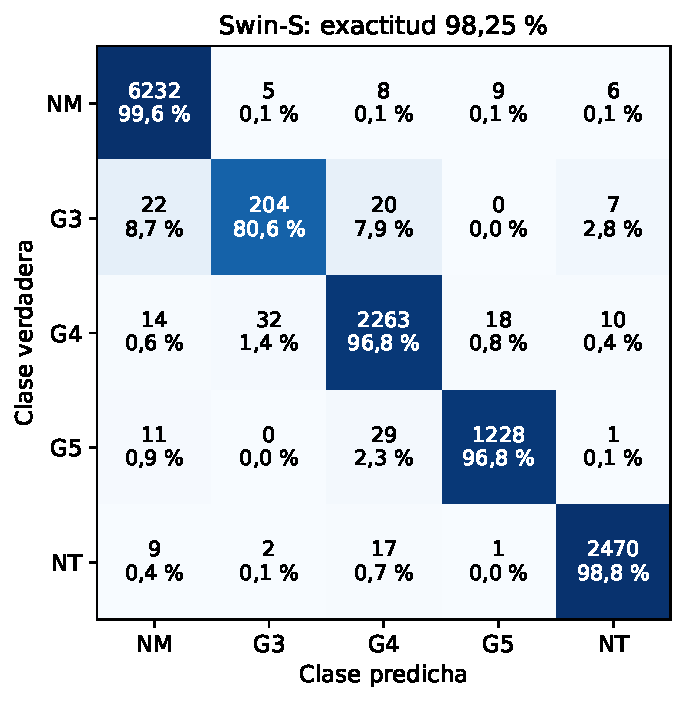
\includegraphics[width=0.5\textwidth]{img/cap09/fig_confusion_5clases_swin.pdf}
  \caption{Matriz de confusión de la clasificación agrupada en cinco categorías (NM, G3, G4, G5 y NT) de Swin-S en el test ID: número de imágenes y porcentaje de cada fila (clase verdadera). Se ha decidido usar la matriz de confusión únicamente del modelo Swin-S, ya que es el que se va a usar como referencia y refleja, de la misma forma que el resto de modelos, los resultados hallados.}
  \label{fig:confusion-5clases}
\end{figure}


\section{Discusión}\label{sec:discusion-clasificacion}

% Puntos para la discusión del capítulo:
% - Swin-S y ConvNeXt-S empatados; ambos por encima de EfficientNetV2-S, ViT-B/16 y ResNet-50 con
%   IC por imagen; con IC por lámina solo se separan claramente de ResNet-50.
% - Las clases minoritarias (glomeruloide, pobremente formadas, Gleason_3) concentran los errores.
% - En la agrupación clínica, Swin-S queda cerca del modelo del artículo.
% - Limitación: el test comparte láminas con el entrenamiento (\cref{cap:fuga}); las métricas miden
%   generalización dentro de lámina, no a pacientes nuevos.
Ha quedado comprobado cómo las arquitecturas modernas (Swin-S y ConvNeXt-S) quedan por encima del resto de modelos, aunque con los IC por lámina solo se separan claramente de ResNet-50, que es el que ha ofrecido los peores resultados. Entre los dos mejores modelos, ha quedado visto que el resultado tiene que considerarse un empate, y se elegirá Swin-S sin que ofrezca ninguna ventaja clara. Ambos han llegado a acercarse a los resultados ofrecidos en~\cite{ayensa2026}. Los procesos de entrenamiento, por lo general, han concluido sin sobreajuste. La particularidad viene de ResNet-50, que presenta un comportamiento anómalo, probablemente debido a la parada temprana. Todos los modelos mejoran en la clasificación binaria y, respecto a la clasificación por categorías, G3 es la que presenta mayores dificultades.
% Cifras: exactitud con IC por lámina (results_fase1/resumen.md): Swin-S {0,9589; 0,9768}, ConvNeXt-S
% {0,9571; 0,9748}, EfficientNetV2-S {0,9412; 0,9645}, ViT-B/16 {0,9391; 0,9631}. Artículo (XCiT-M):
% 97,33 % (14 clases), 98,34 % (5 categorías), 99,25 % (binario); Swin-S 96,88 %, 98,25 %, 99,33 %;
% ConvNeXt-S 96,68 %, 98,07 %, 99,25 %.

\endinput
